%! TEX root = ../thesis.tex
\section{Predikon}
\label{app:sec:predikon}

To make the research presented in Chapter~\ref{ch:predikon} available to the general public, we developed Predikon~\footnote{\href{https://www.predikon.ch}{https://www.predikon.ch}}, a website predicting Swiss referendum votes in real time.
Four times a year, Swiss citizens are called to vote on referenda and popular initiatives.
They can send their ballot remotely or come to the ballot office, on the date of the vote, to deposit it.
Then, starting at 12pm, officials in Swiss municipalities start counting the ballots and report the results as soon as they finish.
We make predictions using the partial national results, \textit{i.e.}, using only the results in the municipalities that are done counting and have reported their results.
In Figure~\ref{app:fig:predikonhome}, the homepage of Predikon shows the predictions in real time for current votes and those of past votes.
We built an interactive tool to visualize the projections of the municipalities in the latent ideological space of Section~\ref{pdk:sec:swiss_referenda}, with PCA (see Figure~\ref{app:fig:predikonpca}) and t-SNE (see Figure~\ref{app:fig:predikontsne}).

\begin{figure}
	\centering
	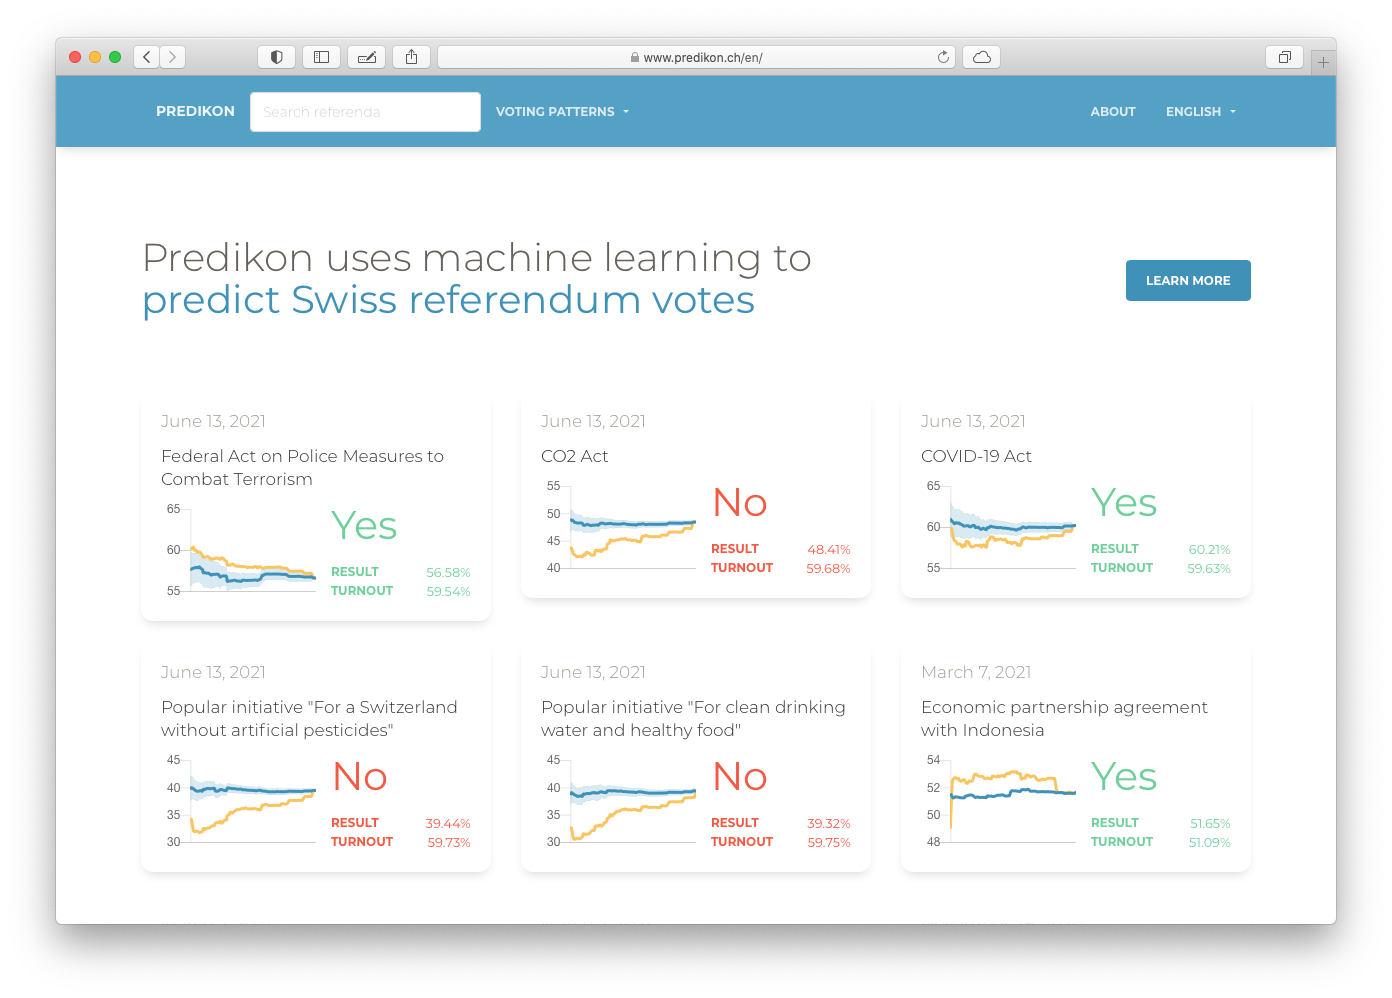
\includegraphics[width=\textwidth]{pdk-home}
	\caption{Home page of Predikon showing predictions of past votes.}
	\label{app:fig:predikonhome}
\end{figure}

\begin{figure}
	\centering
	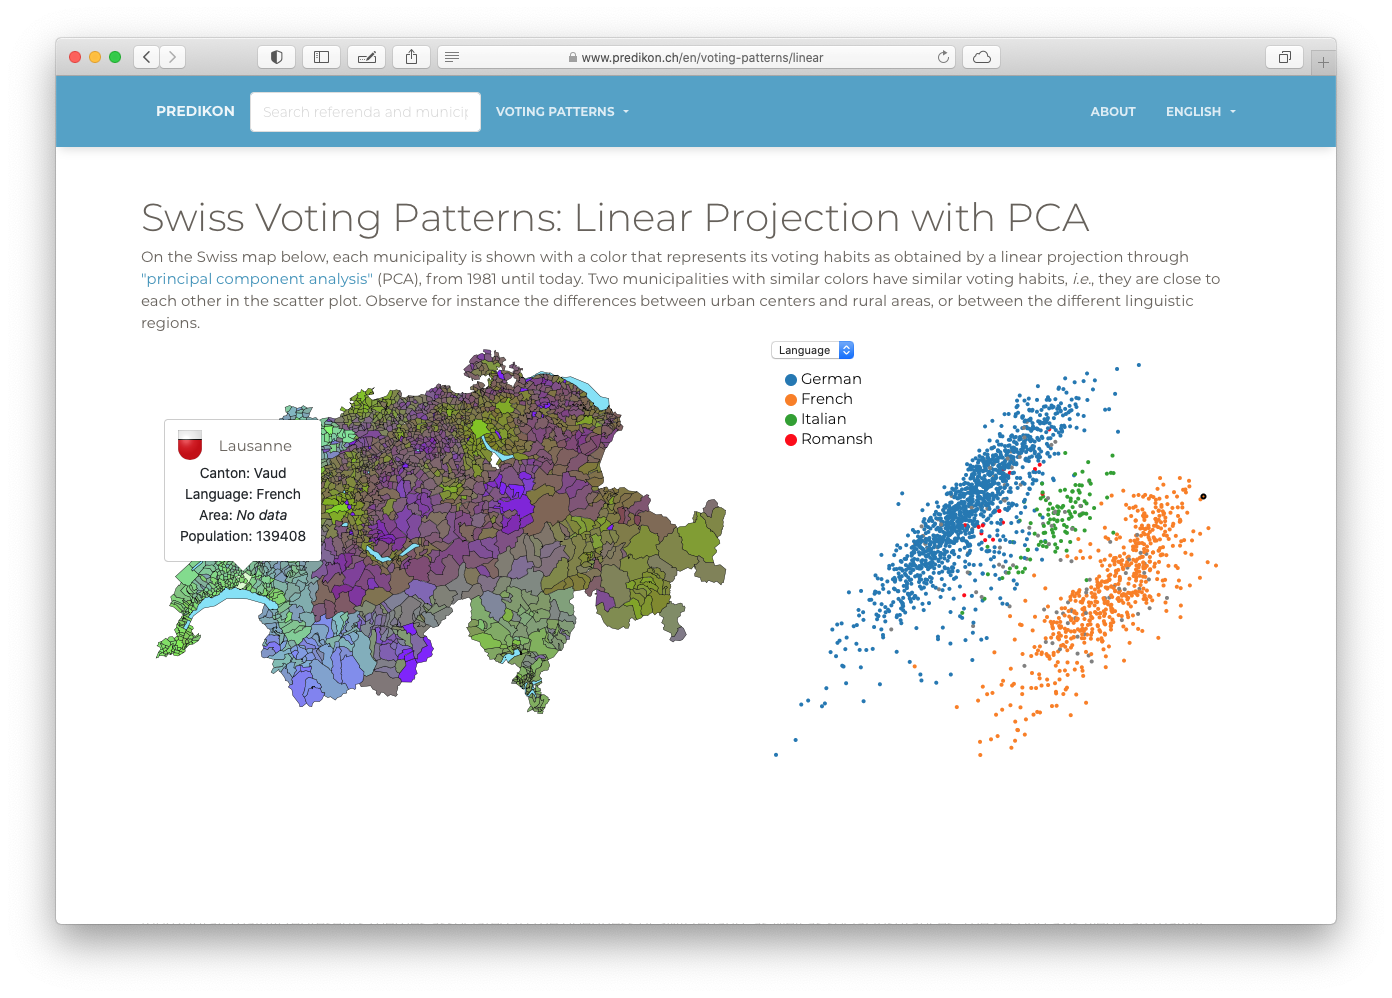
\includegraphics[width=\textwidth]{pdk-pca}
	\caption{Projection of municipalities in ideological space using PCA.}
	\label{app:fig:predikonpca}
\end{figure}

\begin{figure}
	\centering
	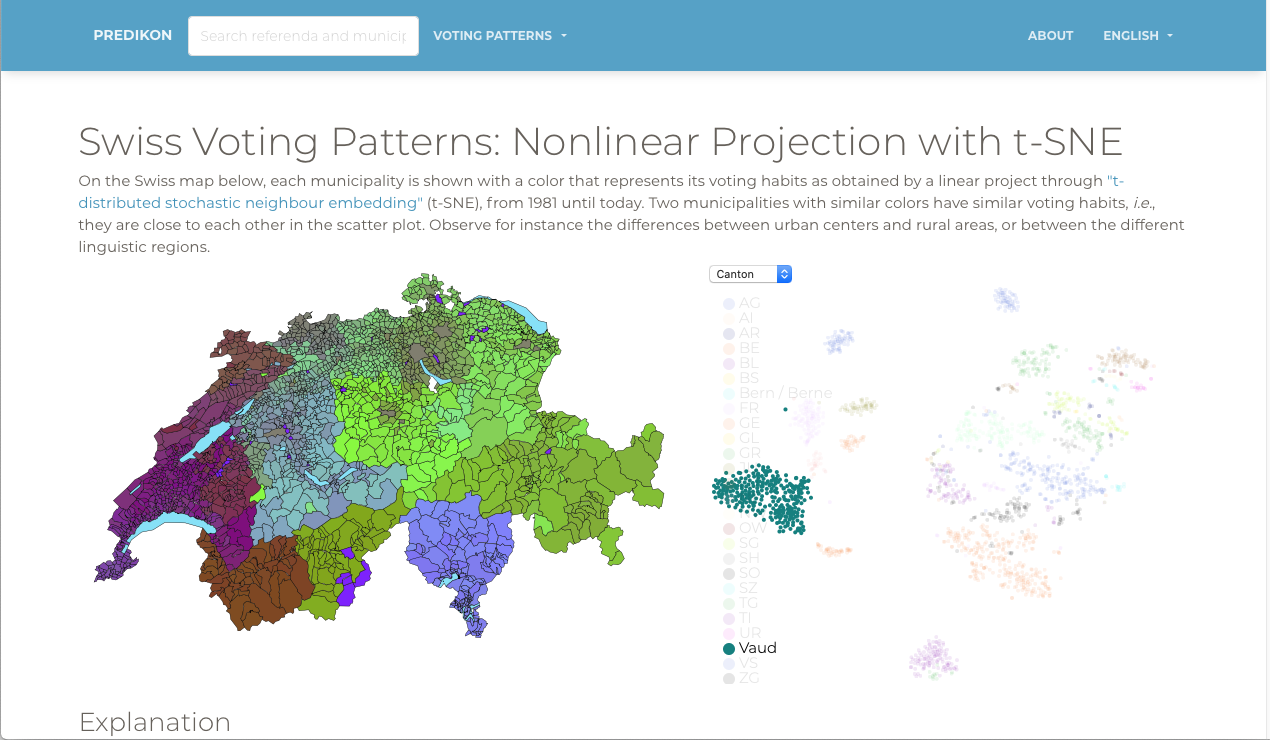
\includegraphics[width=\textwidth]{pdk-tsne}
	\caption{Projection of municipalities in ideological space using t-SNE.}
	\label{app:fig:predikontsne}
\end{figure}
